\documentclass[a4paper, 12pt, onecolumn, openany]{report}

\usepackage[utf8]{inputenc} % Encodage UTF-8
\usepackage[T1]{fontenc}
\usepackage{graphicx}
\usepackage{fancyhdr}
\usepackage[francais]{babel}

\pagestyle{empty}

\title{\bsc{Thème : La Mesure} \\ \Huge{Illusions et effets d'optique}}
\author{Valentine \bsc{Sénégas}, Paul \bsc{Souchon} et Christophe \bsc{Néraud}}
\date{Années 2014 -- 2015}

\begin{document}

\maketitle

\newpage
~
\newpage

\chapter*{Remerciements}
\pagestyle{fancy}
%\lhead{Valentine, Paul et Christophe}
%\chead{}
%\rhead{\textbf{1ère S}}
%\cfoot{\thepage}

\renewcommand{\contentsname}{Sommaire} % Transforme "Table des matières" en "Sommaire"
\tableofcontents

\part*{Illusions et effets d'optique\markboth{Illusions et effets d'optique}{}}
\addcontentsline{toc}{part}{Illusions et effets d'optique}
\chapter*{Introduction\markboth{Introduction}{}}
\addcontentsline{toc}{chapter}{Introduction}
	Nous sommes, tous les jours étonnés par diverses choses qui ne nous apparaissent pas telles qu’elles le sont véritablement. L’œil humain est en permanence trompé par la forme, la taille ou même la distance qui le sépare d’un objet. On appelle cela un effet d’optique.  
	
	Nous étions intrigués et nous nous demandions comment cela était possible, si c’était bien réel. Nous nous sommes alors posés les questions suivantes :
	
	Quelle est la différence entre effet d'optique et illusion ?

	Comment le cerveau interprète-t-il une image ? 
	
	Comment le cerveau peut-il être trompé par une illusion ou un effet d'optique ?
	
	Nous avons tenté de répondre à ces questions en réalisant une expérience : nous avons représenté une situation type où l’image perçue par le cerveau est différente de celle perçue dans la réalité. A travers notre expérience, nous allons ainsi étudier l’image et découvrir par la suite le fonctionnement de l’œil et du cerveau humain, et pourquoi l’interprétation de l’image par l’être humain est différente. Nous verrons dans un dernier temps divers autres types d’effet d’optique.
	
\chapter*{Les yeux, le cerveau et l'image\markboth{Les yeux, le cerveau et l'image}{}}
\addcontentsline{toc}{chapter}{Les yeux, le cerveau et l'image}
	\section*{Composition de l'oeil\markboth{Composition de l'oeil}{}}
\addcontentsline{toc}{section}{Composition de l'oeil}
	L’œil est l’organe de la vision. Le système visuel nous permet de différencier les formes, les tailles, les couleurs ou encore les textures des objets mais également de les situer dans l’espace et de les différencier les uns par rapport aux autres. 
	
	Les déplacements ou encore la vitesse des objets peuvent également être détectés et cela aussi bien le jour que 
la nuit.	

	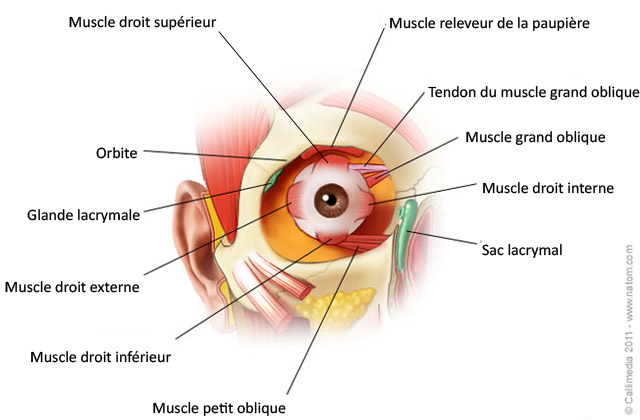
\includegraphics[scale=0.5]{oeil.jpg}
	
	L’œil d’un être humain adulte est une sphère qui mesure environ 2,5 cm de diamètre, et pèse environ 7 grammes. 
	
	La partie antérieure visible ne représente qu’un sixième de l’œil, le reste est situé dans l’orbite et est entouré de graisse. 
	
    Des structures interviennent dans la protection de l’œil et permettent sont fonctionnement :
    \begin{itemize}
   	\item[$\bullet$] Sourcils : ils permettent de protéger l’œil des gouttes de sueur en provenance du front ainsi que de la lumière,
	\item[$\bullet$] Paupières : les paupières mobiles clignent par reflexe toutes les 3 à 7 secondes, elles peuvent également cligner automatiquement lorsqu’un corps étranger arrive dans l’œil ou un soufflement d’air.  Elles protègent l’œil de tous les corps étrangers et permettent également de prévenir la dessiccation (déshydratation de l’œil) car ainsi, les sécrétions telles que le mucus, les larmes, l’huile se répandent à la surface du globe oculaire, son hydratation est alors permanente.  
	\item[$\bullet$] Conjonctive : elle tapisse le blanc de l’œil ainsi que les paupières produisant un mucus lubrifiant.
	\item[$\bullet$] Glande lacrymale : elle sécrète des larmes qui sont répandues sur la surface du globe oculaire grâce aux clignements des yeux, et vont ainsi protéger, nettoyer, humecter et lubrifier la surface de l’œil.
	\end{itemize}	
	
	Chaque globe oculaire est mobile grâce à des muscles fixés dans l’orbite, cavité osseuse du crâne. Ils partent du fond de l’œil et s’attachent sur les côtés du globe oculaire. 
	
    Ces muscles permettent ainsi le mouvement rapide des yeux qui peut aller dans toutes les directions, ils sont au nombre de six, quatre sont droits et deux obliques :        
    \begin{itemize}
    \item[$\bullet$] Le droit supérieur, permet à l’œil de se déplacer vers le haut
	\item[$\bullet$] Le droit inférieur, permet de se déplacer vers le bas
	\item[$\bullet$] Le droit médian (ou interne), permet le déplacement de l’œil vers le nez
	\item[$\bullet$] Le droit latéral (ou externe), permet le déplacement de l’œil vers la tempe
	\item[$\bullet$] L’oblique supérieur (ou grand oblique) Le muscle releveur de la paupière supérieure. 
	\item[$\bullet$] L’oblique inférieur (ou petit oblique) 
	\end{itemize}		
    Trois enveloppes emboitées limitent l’œil humain, la sclérotique, la choroïde et la rétine se prolongeant par le nerf optique :
    \begin{itemize}
	\item[$\bullet$] Sclérotique : c’est une enveloppe opaque et blanche très résistante. Elle devient transparente et forme la cornée à l’avant de l’œil, la face visible. Le rayon de courbure et alors plus petit. Sa netteté va être assurée grâce aux larmes et clignements de l’œil.
	\item[$\bullet$] Choroïde : elle recouvre entièrement la sclérotique et est noire ainsi que vascularisée. Elle devient l’Iris colorée présentant une ouverture à l’avant de l’œil, la pupille.  
	\item[$\bullet$] Rétine ($0,2 \; mm$) : c’est l’enveloppe la plus interne de l’œil, c’est un tissu nerveux grisâtre, mince, collé contre la choroïde et se prolonge par le nerf optique. 
	\end{itemize}	
Avant d’atteindre le fond de l’œil, les rayons lumineux doivent traverser des milieux transparents le contenant :
	\begin{itemize}
	\item[$\bullet$] L’humeur aqueuse a une composition semblable à celle du plasma sanguin et remplit l’espace entre la cornée et le cristallin.
	\item[$\bullet$] Le cristallin, biconvexe, se trouve derrière la pupille et va se déformer grâce à l’action de petits muscles permettant ainsi de modifier sa convexité.
	\item[$\bullet$] L’humeur vitrée est en arrière du cristallin. C’est une substance gélatineuse remplissant l ‘espace compris entre le cristalline et la rétine.
	\end{itemize}
	
	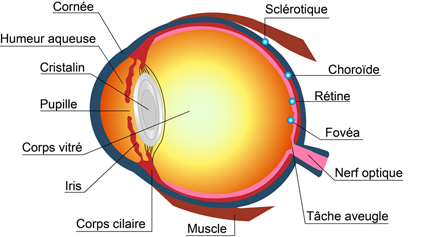
\includegraphics[scale=0.8]{schema_oeil.jpg}

	\section*{Fonctionnement de l'oeil\markboth{Fonctionnement de l'oeil}{}}
\addcontentsline{toc}{section}{Fonctionnement de l'oeil}
		\subsection*{Propagation de la lumière\markboth{Propagation de la lumière}{}}
\addcontentsline{toc}{subsection}{Propagation de la lumière}
		Dans un milieu transparent, homogène et isotrope (c’est-à-dire qui a les mêmes propriétés dans toutes les directions), la lumière se propage en un mouvement rectiligne et uniforme.
		
	Dans le cas où le milieu n’est pas homogène, par exemple lors d’une différence de température, la lumière est déviée : c'est le phénomène de réfraction. Lorsque la lumière traverse un milieu transparent, elle subit ce phénomène. C’est le cas par exemple de l’eau ou encore l'air. 
	
	Ce sont les lois de Snell-Descartes qui définissent les angles de réfraction. Prenons un exemple : un rayon de lumière, appelé rayon incident, se déplace dans un premier milieu transparent, l'air. Ce rayon traverse ensuite un second milieu transparent, l'eau. Le rayon arrive à la surface de l'eau avec un certain angle par rapport à la normale : c'est \textit{l'angle d'incidence}, note $i$. Lorsque le rayon traverse l'eau, il est dévié par rapport à la normale. L'angle ici présent est \textit{l'angle de réfraction}, noté $r$, ou parfois $i_{2}$.
	
	Chaque milieu transparent possède un indice de réfraction, noté $n_{milieu}$, différent. Il est pour l'air de $n_{air} = 1,0003$, et pour l'eau de $n_{eau} = 1,333$.
	
	Nous pouvons calculer les angles d'incidence et de réfraction, ou bien les indices de réfraction de différents milieux transparents grâce à la formule :	
	\[
	n_{1} \cdot \sin i = n_{2} \cdot \sin r
	\]	
	La réfraction d’un rayon lumineux, ainsi que la manière dont il est dévié, est donc plus ou moins forte en fonction du milieu qu’il traverse, ainsi qu’en fonction de l’angle d’incidence.
	
	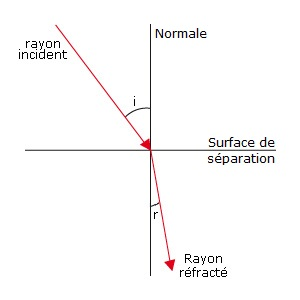
\includegraphics{refraction.jpg}
	
	 En plus du phénomène de réfraction, la lumière subit un phénomène de dispersion. Par exemple, si un faisceau de lumière blanche est dirigé vers une surface plane d'un bloc de verre, elle est décomposée lors de sa réfraction : le spectre de la lumière blanche apparaît.
	 
	 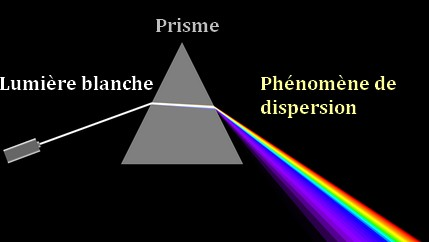
\includegraphics[scale=0.73]{dispersion.jpg} 
	 
	 La dispersion est à l’origine des arc-en-ciel : la lumière passe à travers des gouttes d’eau, qui dispersent la lumière, et font apparaître le spectre de la lumière blanche. 

		\subsection*{Formation d'une image\markboth{Formation d'une image}{}}
\addcontentsline{toc}{subsection}{Formation d'une image}
		L’œil est un organe, disposant d’une rétine qui tapisse son fond, dont le but est de former une image à partir de rayons de lumière puis de l’envoyer au cerveau afin qu’il la traite. En plus d’être capable de détecter la lumière, l’œil doit aussi pouvoir détecter sa direction. 
		
	Tout d’abord, nous allons nous intéresser à la formation d’une image dans un milieu quelconque.
	
	Lorsqu’un objet est éclairé par une source lumineuse, des rayons de lumière se forment. Lorsque l’on intercale une lentille convergente entre ces rayons, nous constatons qu’ils convergent en un point.
	
	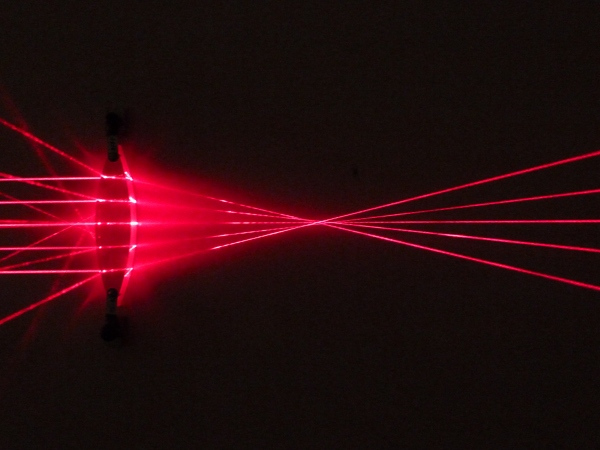
\includegraphics[scale=0.4]{lentille_convergente.jpg}
		
	Si l’on positionne un écran après le foyer image, on constate l’apparition d’une image dessus : c’est l’image formée à partir de l’objet. En fonction de l’endroit où se situe l’objet par rapport à la lentille, l’image sera plus ou moins grande, et plus ou moins éloignée de la lentille. Aussi, elle est toujours renversée. 
	
	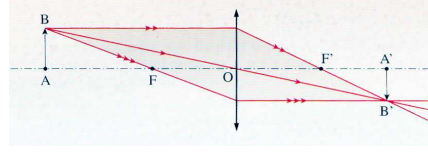
\includegraphics[scale=1]{formation_image.png}
		
		La formation d’une image suit trois règles :
		\begin{itemize}
		\item[$\bullet$] Si l’objet est situé à l’infini, l’image se forme au foyer,
		\item[$\bullet$] Si l’objet est situé à la distance focale, l’image est située à l’infini,
		\item[$\bullet$] Si la distance entre la lentille et l’objet est supérieure à la distance focale, l’image est située après la lentille, et est renversée.
		\end{itemize}
		
	Dans le cas d’une loupe, l’objet est situé après le foyer objet, l’image est dans le bon sens, et se forme avant l’objet : c’est une image virtuelle.

		\subsection*{L'oeil\markboth{L'oeil}{}}
\addcontentsline{toc}{subsection}{L'oeil}
		L’œil est composé d’un cristallin, qui peut être assimilé à une lentille convergente. Lorsque les rayons lumineux provenant d’un objet éclairé y pénètrent, ils convergent donc en un point. L’image formée à partir de l’objet est une image inversée.
		
		Lorsqu’un objet est éclairé, nous pouvons le voir. En effet, les rayons lumineux qui en proviennent passent à travers l’iris, et rentrent dans l’œil. Ils subissent une réfraction lorsqu’ils traversent l’humeur vitrée et aqueuse, et peuvent donc former l’image renversée sur la rétine.
		
	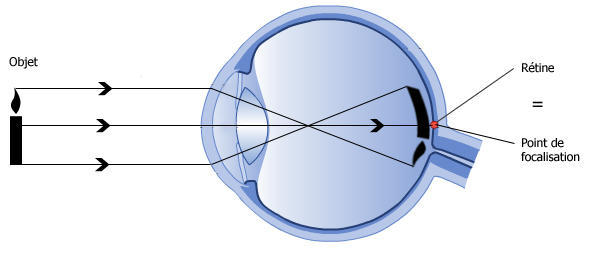
\includegraphics[scale=0.2]{rayons_lumineux.jpg}
		
	L’œil dispose d’un système d’accommodation. Il est sur ce point assimilable à un appareil photo, qui possède une fonction de mise au point. Pour l’œil, le cristallin se déforme plus ou moins. Par exemple, plus un objet est proche, et plus le cristallin va se courber. Par conséquent, sa distance focale diminue, et sa vergence augmente. 
	\newpage
	L’œil est un organe pouvant posséder des défauts.

	\subsubsection*{La myopie}
	L’œil est trop convergent, et les images se forment avant la rétine. Le positionnement d’une lentille divergente devant l’œil peut corriger ce problème.
	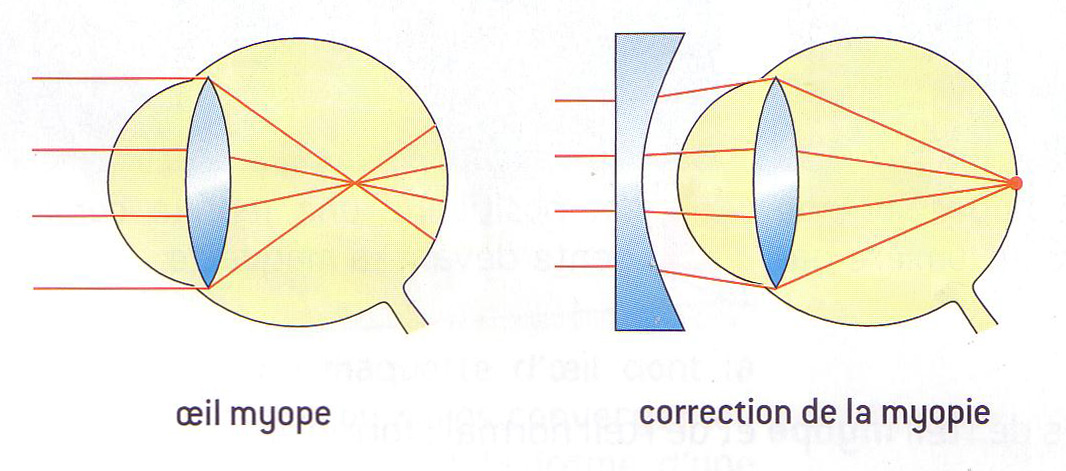
\includegraphics{myopie.jpg}
	
	\subsubsection*{L'hypermétropie}
	C’est le contraire de la myopie, l’œil n’est pas assez convergent, et donc les images se forment après la rétine. Il faut cette fois-ci placer une lentille convergente devant l’œil.
	
	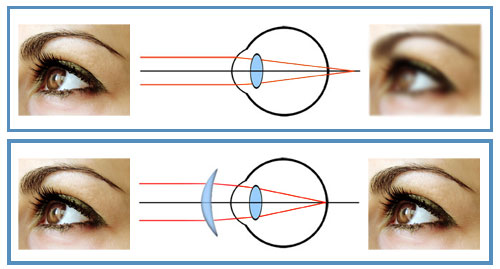
\includegraphics[scale=0.5]{hypermetropie.jpg}
	
	\subsubsection*{La presbytie}
	C’est un défaut de l’œil qui apparaît en général chez les personnes âgées. En effet, le cristallin est « fatigué », il ne peut plus accommoder. De ce fait, les images de près se forment derrière la rétine. Il faut cette fois également porter des lunettes convergentes.
	
	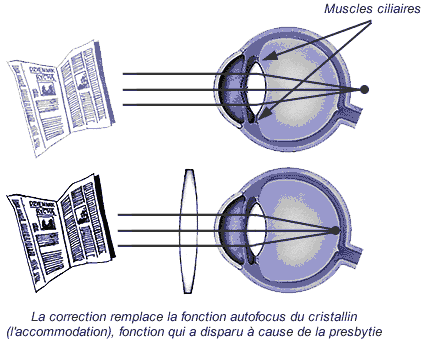
\includegraphics[scale=0.7]{presbytie.png}
	
	\subsubsection*{L'astigmatisme}
	C’est un défaut de la composition de l’humeur aqueuse et/ou de l’humeur vitrée. Les rayons qui les traversent ne forment plus un point lumineux sur la rétine, mais une tache de dimension et de formes variées.
	
	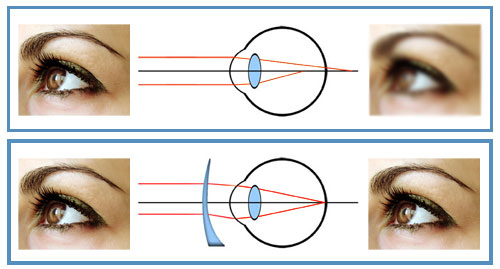
\includegraphics[scale=0.5]{astigmatisme3.jpg}
	
	\newpage
	
	À présent, intéressons-nous à la sensibilité de l’œil à la lumière.
	
	La rétine est un tissu nerveux, c’est un prolongement du cerveau. Elle est composée de cellules photosensibles, soit sensibles à la lumière. Ces cellules peuvent être de deux types : des cônes et des bâtonnets. Les cônes détectent les couleurs, et les bâtonnets sont sensibles aux faibles intensités lumineuses. Il existe une zone située au centre de la rétine, la fovéa, dont chacune des cellules est reliée à une seule cellule nerveuse. C’est cette zone qui est à l’origine de l’acuité visuelle (le fait de voir nettement un petit objet lointain), car chacune des cellules la composant captera un point lumineux différent de celui capté par les autres cellules.
	
	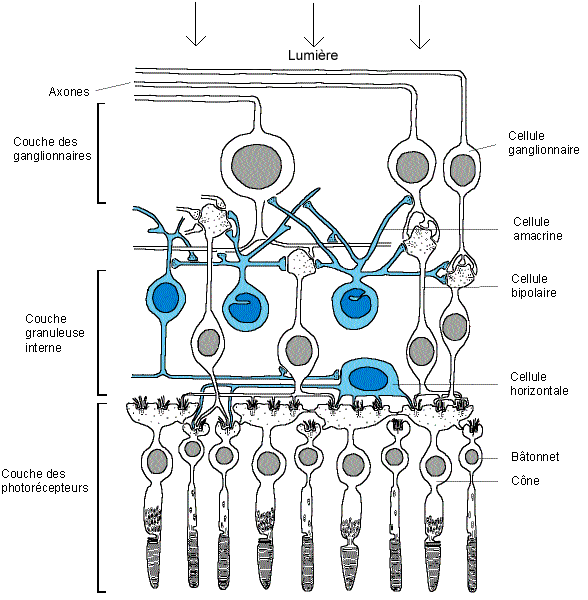
\includegraphics[scale=0.5]{retine.png}
	
	Lorsqu’on s’éloigne de la fovéa, les cellules photosensibles sont reliées à une seule cellule nerveuse. L’œil possède en fait un champ de vision net réduit par rapport à la taille de la rétine.
	
	Les cônes sont sensibles soit au vert, au rouge ou au bleu. C’est ainsi que l’œil va pouvoir détecter toutes les couleurs, grâce à la combinaison de ces cônes. Les bâtonnets, quant à eux, ne peuvent détecter que le noir et le blanc, mais sont sensibles aux faibles luminosités : c’est ce qui fait qu’on dispose d’une vision nocturne, et donc que nous n’y voyons pas de couleurs.
	
	Toutes les cellules photosensibles sont reliées à des cellules nerveuses, qui sont elles-mêmes reliées aux cellules du nerf optique. Par conséquent, il n’y a pas de cellules photosensibles à l’endroit où le nerf optique arrive à la rétine. Cette zone ne détecte pas la lumière, c’est la tâche aveugle.
	
	Après avoir découvert le fonctionnement de l’œil, nous allons nous intéresser à celui du cerveau dans le cadre de la vue.

	\section*{Fonctionnement du cerveau dans le cadre de la vue\markboth{Fonctionnement du cerveau dans le cadre de la vue}{}}
\addcontentsline{toc}{section}{Fonctionnement du cerveau dans le cadre de la vue}
	Le cerveau est l’organe central du corps humain. C’est lui qui contrôle le fonctionnement des autres organes.Dans le cadre de la vue, il est capable de recevoir un message nerveux provenant de l’œil, plus précisément de la rétine, par le nerf optique, qui contient une image captée par l’œil, et de l’interpréter.
	
	C'est par le sens de la vue que nous percevons la lumière, les formes et les couleurs, que nous apprécions les détails des objets, leur distance et leur relief.
	
	Les informations visuelles recueillies par l'œil sont transformées en messages nerveux au niveau de la rétine, puis transmit par les nerfs optiques jusqu'au cerveau. C'est alors le cortex visuel qui analyse le stimulus reçu, élabore la perception visuelle et répond de façon appropriée.
	
	Comment une image est-elle transmise par l’œil au cerveau ? Comment celui-ci l’interprète ?

		\subsection*{Transmission de l'image\markboth{Transmission de l'image}{}}
\addcontentsline{toc}{subsection}{Transmission de l'image}
		Tout d'abord il faut savoir que  l'œil est mobile grâce à des muscles fixés dans l'orbite. C'est un système optique qui permet la formation d'une image réelle, et surtout  renversée par rapport à l'objet regardé.  
	
	L'intérieur des globes oculaires est rempli de différents milieux transparents jouant le rôle d'une lentille, qui permettent donc la formation d'une image au fond de l'œil. Il s'agit de l'humeur aqueuse, du cristallin et de l'humeur vitrée.
	
	Entre l'iris et la cornée se trouve un espace rempli d'humeur aqueuse, un fluide semblable à l'eau.
	
	Ensuite derrière l'iris se trouve le cristallin, une lentille transparente biconvexe (offrant deux faces arrondies opposées) qui permet de faire la « mise au point » pour des objets rapprochés.
	
	Comment l'image parvient-elle au cerveau ?
	
	L'absorption de lumière par les pigments photosensibles des cônes et des bâtonnets modifie leurs propriétés électriques et conduit à la naissance d'un message nerveux. En effet, si la stimulation visuelle est suffisante, un message nerveux, constitué d'une succession de signaux électriques, est généré dans les fibres du nerf optique. Une variation de l'intensité du stimulus visuel se traduit alors par une variation de la fréquence des signaux électriques.
	
	Les messages nerveux visuels générés par la rétine sont acheminés par les nerfs optiques jusqu'au cerveau.
	
	Le nerf optique de l'œil droit et celui de l'œil gauche se croisent au niveau du chiasma optique. À cet endroit, la moitié des fibres de chacun des nerfs optiques s'entrecroisent et passent dans l'hémisphère opposé. Les autres fibres rejoignent directement le lobe occipital du cerveau, où se trouvent les centres d'interprétation de la vision. Ainsi, chaque hémisphère reçoit des informations visuelles issues des deux yeux.
		
	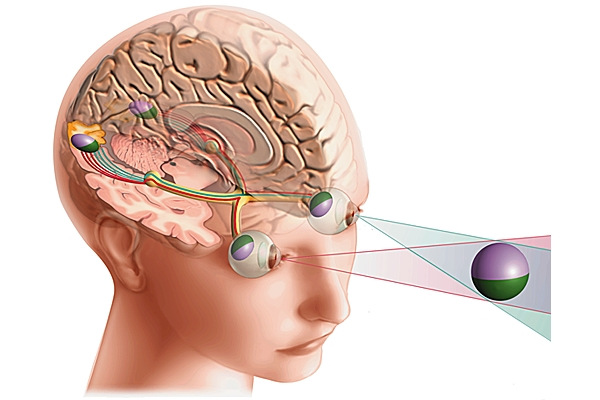
\includegraphics[scale=0.7]{deux_yeux.jpg}		
	
	Il existe une zone de relais, située entre le chiasma optique et le cortex visuel, dans laquelle toutes les fibres des nerfs optiques sont en connexion synaptique avec d'autres neurones qui conduisent les messages jusqu'au cortex visuel. La transmission du message nerveux se fait alors par l'intermédiaire de substances chimiques, les neurotransmetteurs.
	
	Ainsi, certaines substances hallucinogènes, en se fixant sur les récepteurs de ces neurotransmetteurs, modifient la perception visuelle.

		\subsection*{Interprétation de l'image\markboth{Interprétation de l'image}{}}
\addcontentsline{toc}{subsection}{Interprétation de l'image}
		Différentes régions du cerveau sont impliquées dans le processus de la vision : le cortex visuel primaire mais aussi différentes aires cérébrales spécialisées.
		
	Après avoir franchi la zone de relais, la plupart des messages nerveux visuels arrivent dans une aire située à l'arrière du cortex occipital de chacun des deux hémisphères. Ces deux aires cérébrales forment le cortex visuel primaire. Chacune d'entre elles reçoit des informations provenant des deux yeux. Ainsi, toute lésion située dans cette zone provoque une cécité plus ou moins prononcée. Parallèlement, certaines informations visuelles arrivent directement dans différentes aires visuelles spécialisées dans le traitement de la couleur, des formes ou encore des mouvements.
	
	Ainsi, toutes les informations concernant une image sont traitées en parallèle. Leur intégration et les échanges entre l'ensemble de ces aires permettent ensuite d'avoir une perception globale et unifiée.
	
	Les gènes interviennent dans l'organisation et la structure du cortex visuel et sont, par conséquent, impliqués dans la perception visuelle. Ces structures sont similaires chez tous les individus, ce qui donne initialement à chacun les mêmes potentialités visuelles.
	
	À condition d'être stimulées, les capacités visuelles se développent entre 0 et 10 ans, en même temps que le cerveau.
	
	En outre, l'environnement et l'expérience individuelle ont une influence sur les structures corticales mises en jeu dans la vision.
	
	Le cortex est divisé en plusieurs aires corticales spécifiques (V1, V2, V3, V4 et V5). Il n'est pas nécessaire d'expliquer la fonction de ces aires corticales car cela ne nous intéresse pas, or on peut ajouter que l'aire corticale V4 est chargée du traitement des formes et des couleurs.

\chapter*{Comment le cerveau peut-il être trompé ?\markboth{Comment le cerveau peut-il être trompé ?}{}}
\addcontentsline{toc}{chapter}{Comment le cerveau peut-il être trompé ?}
	\section*{Présentation de notre illusion\markboth{Présentation de notre illusion}{}}
\addcontentsline{toc}{section}{Présentation de notre illusion}
	\section*{Explication de l'illusion : comment l'a-t-on construite et pourquoi est-ce une illusion ?\markboth{Explication de l'illusion}{}}
\addcontentsline{toc}{section}{Explication de l'illusion}
\chapter*{Autres exemples d'illusion\markboth{Autres exemples d'illusion}{}}
\addcontentsline{toc}{chapter}{Autres exemples d'illusion}
	\section*{Différence entre illusion et effet d'optique\markboth{Différence entre illusion et effet d'optique}{}}
\addcontentsline{toc}{section}{Différence entre illusion et effet d'optique}
	\section*{Mirages\markboth{Mirages}{}}
\addcontentsline{toc}{section}{Mirages}
	\section*{Stéréogrammes\markboth{Stéréogrammes}{}}
\addcontentsline{toc}{section}{Stéréogrammes}
	Les stéréogrammes sont des images en 3 dimensions où sont dissimulées des formes. Ils apparaissent sous forme d’une texture abstraite, mais avec un agencement particulier, qui permet de faire apparaître la forme recherchée.
	
	Il existe manières de les voir : il faut placer son visage le plus près possible de l’image. En effet, lorsqu’on regarde une image ou un objet, nos yeux sont focalisés sur un point situé derrière l’image. L’image reçue par chaque œil est différente, mais le cerveau les interprète comme si c’étaient les mêmes. Le cerveau est capable de reconstituer le relief caché dans le stéréogramme, mais seulement si on se focalise dessus. Se placer très près de l’image fait que les yeux ne peuvent plus faire le point, ils regardent alors le vide. Ensuite, il faut reculer doucement, toujours en gardant le même type de vision. 
	
	Voici un exemple de stéréogramme :
\end{document}
